\section{R\&D of ILD MUON SYSTEM}

\subsection{Introduction}
The main goals of the Muon System in the ILC Detector are the identification of the muons from the interactions and recover the energy leakage out of the hadron calorimeter (Energy Tail Catcher).
The muon system/tail catcher detector instruments the iron return yoke in the barrel and in the forward regions. The yoke barrel part is equipped with one sensitive layer in front of the iron yoke, 10 layers spaced 14 cm apart, followed by three sensitive layers spaced by \unit[60]{cm} apart. The forward part of the yoke is equipped with 10 layers spaced by \unit[14]{cm}, followed by two sensitive layers spaced by \unit[60]{cm.} The overall layout of the muon system/tail catcher is shown in Figure~\ref{fig:Muon:ILDMuon:schematic}

\begin{figure}
	\centering
	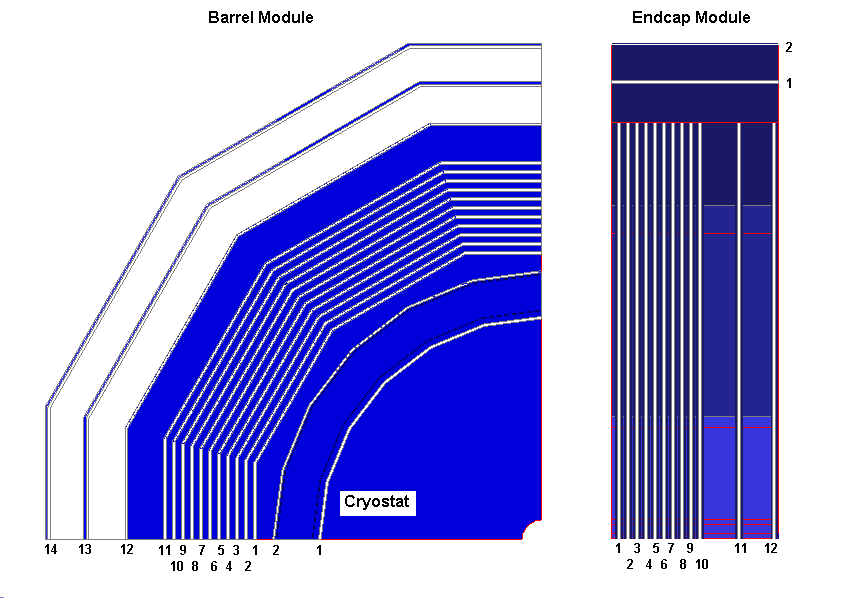
\includegraphics[width=.5\textwidth]{MuonDetector/MuonDetectorILD/muonSchematic}
	\caption{The structure of the sensitive Layers of the Muon System /Tail Catcher for the Barrel and End Cap Parts}
	\label{fig:Muon:ILDMuon:schematic}
\end{figure}

Two main options are investigated for the sensitive layers, scintillator strips equipped with wave-length shifting fibres and readout with silicon photomultipliers (SiPM), or resistive plate chambers (RPC).
The requirement that the muon system/tail catcher serves both as a muon tracker and as a tail catcher impacts its design. The first section of the system provides ten relatively closely spaced layers, to act as a reasonable calorimeter. Mechanical constraints limit the iron thickness between readout stations to be at least 10 cm. At the rear of the muon system the distance between stations in much increased, since they only need to act as a muon tracker. Three layers in the barrel, two in the endcap are spaced \unit[60] cm apart. The fact that the coil adds about two interaction lengths of material in front of the muon system limits the effect of the tail catcher. To maximize its impact a sensitive layer is placed in front of the iron yoke, directly behind the coil and the first 10 layers are spaced more closely to improve the calorimetric performance of the system.
With the anticipated point resolution of about \unit[1]{cm} and the current design, the
achievable momentum resolution for muons is limited by multiple scattering up to
momenta of \unit[5]{GeV}. However in particular for muons inside jets the addition of the
information from the muon system/tail catcher can significantly improve the purity of the muon sample.
The main option for the sensitive layers will use extruded scintillation strips with a thickness of $7-\unit[10]{mm}$ and a width of $25-\unit[30]{mm}$. A \unit[1]{mm} wide extruded groove running along the center of the strip will take a commercially available wave length shifting (WLS) fibers. The scintillator strips will be covered on the outside by a layer of \ce{TiO2}, that is co-extruded alongside the scintillator during the extrusion process. The maximal length of strips required for ILD is $200-\unit[250]{cm}$. The signals will be readout from both sides of the strips by silicon photo multipliers, coupled to the wave length shifting (WLS) fibers. Reading out both sides of a strip offers the possibility to define the position of the hits along the strip, which will help in reducing the fake rate in the muon system. Figure~\ref{fig:Muon:ILDMuon:sensitive} (left) shows the design of the scintillator strip. The right picture presents the signal (number of photons) of the scintillation strip with WLS and SiPM readout from both sides.

\begin{figure}
	\centering
	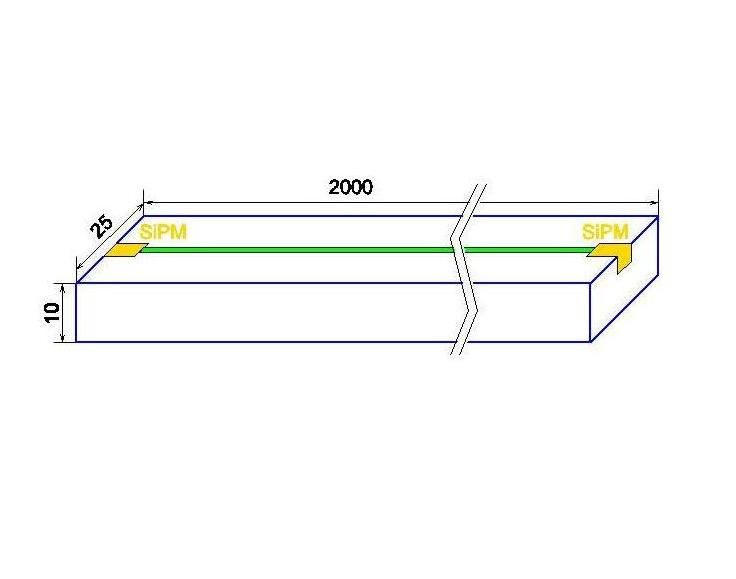
\includegraphics[width=.495\textwidth]{MuonDetector/MuonDetectorILD/muonDetectorSensitiveElements}\hfill
	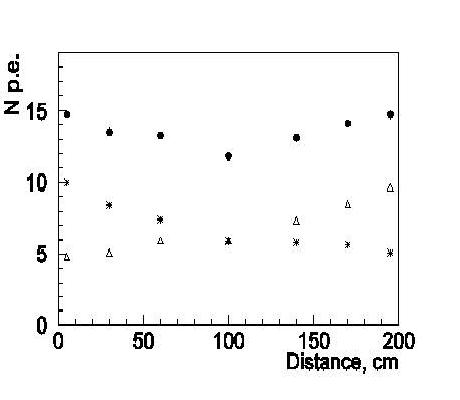
\includegraphics[width=.495\textwidth]{MuonDetector/MuonDetectorILD/muonDetectorSignalReadout}
	\caption{Muon System/Tail Catcher sensitive elements:
left: schematic view of scintillator strip with SiPM readout, right: signal from both sides of the \unit[2]{m} length scintillator strip with WLS and SiPM readout. {\color{red} right-hand figure not referenced in text}}
	\label{fig:Muon:ILDMuon:sensitive}
\end{figure}


Resistive plate chambers (RPC) are considered as an alternative sensitive elements. Main features are excellent granularity up to $1\times\unit[1]{cm^2}$ pads and one
threshold (1-bit) digital readout. Several types of RPCs have been successfully constructed and tested in the worldwide HEP community and within the ILC R\&D program [5].


\subsection{Recent Milestones}
The major R\&D effort of the Muon System/ Tail Catcher Development was concentrated on the optimization of the overall structure of the Muon System/ Tail Catcher:
1.	Detailed Full Monte Carlo Simulation of the Muon System/Tail Catcher, it is concern to choose the geometry of detection plane, geometry of the stereo layers, number of the layers of the detection system and their position, especially concern to the energy leakage,
2.	Study of the performance of the Muon System/Tail Catcher,
3.	Optimization of the detection elements of the Muon System/Tail Catcher. I first this is concern the design of the main detection elements – scintillation strips with the SiPM readout,
4.	Development of the Digital options of the SiPM for the Muon System/Tail Catcher, which will dramatically simplify the readout electronics and data processing.


\subsection{Engineering Challenges}
The main engineering challenge is the build the Distributed Large Scale of the Muon System/Tail Catcher and their embedment in the Solenoid Magnet Yoke. Beginning this year will start the study of the integration of the large scale distributed Muon System/Tail Catcher Detectors in the Structure of the Solenoid Magnet Yoke.

\subsection{Future Plans}
1.	Continue of the optimization of the Muon System/Tail Catcher on base detailed Monte Carlo Simulation and Reconstruction Chain,
2.	Study of the Integration of the Muon System/Tail Catcher in to Solenoid Yoke,
3.	Build of the prototypes of the Muon System/Tail Catcher detection elements on base of the Scintillator Strip/Wavelength Shifter and Analog SiPMs for the study of the main elements as thickness, length, reflection coating, wavelength shifters light yield and other. For this purposes will be develop the test setup for the cosmic muons detection,
4.	Design and Technology development of the Analog SiPMs on base CMOS technology as preliminary options for the Muon System/Tail Catcher optimization,
5.	Technology Development of the Digital option of the SiPMs on base innovative 3D interconnection (3D-IC) technology with fully digital readout and processing electronics.

\subsection{Applications Outside of Linear Colliders}
One of the important application of practically full design and technology of the Muon System/Tail Catcher in the Homeland Security is the Muon Tomography for the transport containers. The checking of the millions of the transport container in present time is one of the crucial and urgent problems, which don’t have the efficient solution. The muon tomography, based on the HEP Muon System could be solution. The development of the Digital SiPMs will have strong impact on the many application areas, in particular to Nuclear Medicine – Positron Emission Tomography.  The new generation of the PET scanners will be developed on base of the All Digital SiPM Readout


{\color{red} References not referred to in text}

[1]	ILD Concept Group, International Large Detector DBD, 2013,
[2]	N. D'Ascenso, N. Saveliev, Mathematical modeling and Study of the ILD Muon System/Tail Catcher", http://www-flc.desy.de/lcnotes
[3]	V. Balagura, M. Danilov, et al., Study of scintillator strip with wavelength shifting fiber and silicon photomultiplier" Nucl.Instrum.Meth. A564 (2006) 596
[4]	C. Adloff et al., Construction and performance of a silicon photomultiplier/extruded scintillator tail-catcher and muon tracker" JINST 7 (2012) 4015, arXiv:1201.1653 [physics.ins-det]
[5]	J. Repond, Overview of the DHCAL Project" arXiv:1005.0412 [physics.ins-det]..
